\item Solid sphere A is rotating about an axis PQ. If the radius of the sphere is 5cm then its radius of gyration about PQ will be \( \sqrt{x} \) cm. The value of x is \underline{\hspace{2.5cm}}.
    \begin{center}
        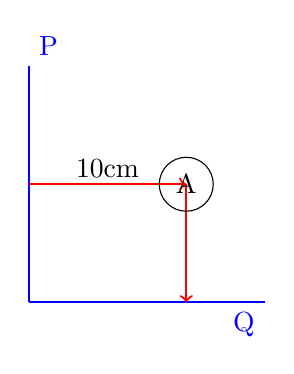
\begin{tikzpicture}
            \draw[blue, thick] (0,0) -- (0,3) node[anchor=south west] {P};
            \draw[blue, thick] (0,0) -- (3,0) node[anchor=north east] {Q};
            \draw[red, thick, ->] (0,1.5) -- (2,1.5);
            \draw[red, thick, ->] (2,1.5) -- (2,0);
            \node at (2, 1.5) [circle, draw=black] {A};
            \node at (1, 1.7) {10cm};
        \end{tikzpicture}
    \end{center}